\documentclass{standalone}
\usepackage{tikz}
\usepackage{tikz-feynman} % Paquete para diagramas de Feynman
\usepackage{amsmath} % Para el símbolo de la llave

\begin{document}

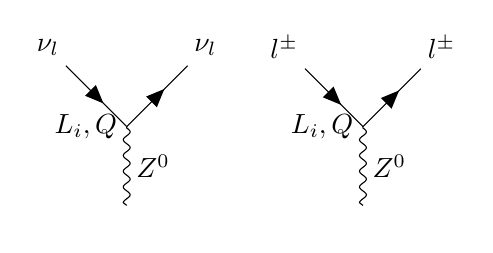
\begin{tikzpicture}
    \begin{feynman}
        \vertex (u) at(-1,1){$\nu_l$};
        \vertex (d) at(1,1){$\nu_l$};
        \vertex (W1) at(0,0);
        \vertex (W2) at(0,-1);
        \node[left] at(0,0){$L_i,Q$};
        \diagram* {
            (u) --[fermion] (W1) --[fermion] (d),
            (W1)--[boson, edge label= $Z^0$] (W2),
        };
        \node[below] at(W2);
    \end{feynman}
    
    \begin{scope}[shift={(3,0)}]
        \begin{feynman}
        \vertex (u) at(-1,1){$l^\pm$};
        \vertex (d) at(1,1){$l^\pm$};
        \vertex (W1) at(0,0);
        \vertex (W2) at(0,-1);
        \node[left] at(0,0){$L_i,Q$};
        \diagram* {
            (u) --[fermion] (W1) --[fermion] (d),
            (W1)--[boson, edge label= $Z^0$] (W2),
        };
    \end{feynman}
    \end{scope}
\end{tikzpicture}

\end{document}
